
\chapter{Second Example}

\section{Introduction}
\blindtext \index{example1}
\cite{Suratekar2018}. 

Second acronym will be \gls{yaa}. This also can be used further as \gls{yaa}. This is example of footnote\footnote{This is footnote.}.
\section{Figure Example}
\blindtext 
\begin{figure}
	\centering
	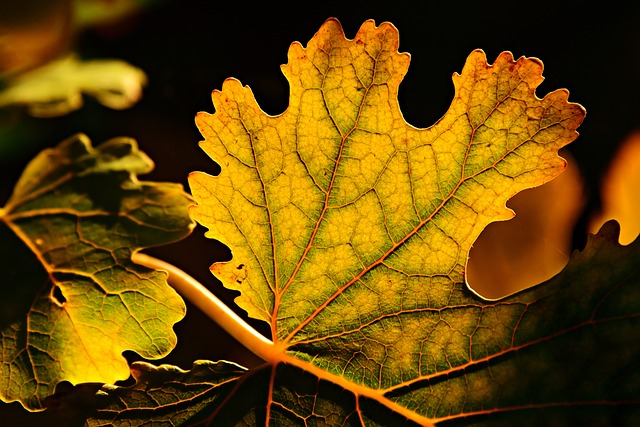
\includegraphics[width=0.7\linewidth]{figs/example}
	\caption{Figure downloaded from Pixabay.com and released under CC0.}
	\label{fig:example}
\end{figure}
\blindtext \index{example1}

\section{Table Example}
\blindtext \index{example2}

\begin{table}
	\centering
\begin{tabular}{|c|c|c|}
	\hline 
1	&  2& ssdfds \\ 
	\hline 
3	& 4 & sdfsdf \\ 
	\hline 
5	& 6 &  sdfsdf\\ 
	\hline 
7	&  8&  sdfsdfsdf\\ 
	\hline 
\end{tabular}
\caption{Example Table} 
\end{table}

\blindtext 

\blindtext 

% After each chapter you can add biblography.
% If you want only one Biblography, remove following helper file and put content of it in main.tex
\clearpage
% This is helper file which you can use in every chapter if you want to have separate biblography for each chapter

% If you want only single biblography for all thesis, just copy paste following content at the end of main.tex

	\bibliographystyle{unsrt}
	\bibliography{main_ref}
	